\documentclass[11pt]{article}
\usepackage[margin=1in]{geometry}
\usepackage{graphicx}
\usepackage[font={small, it}]{caption}
\usepackage{matlab-prettifier}
\usepackage{listings}
\usepackage{keystroke}
\usepackage{menukeys}
\usepackage{amsthm}
\usepackage{subfigure}
\lstset{ %
language=Matlab,                % choose the language of the code
basicstyle=\footnotesize,       % the size of the fonts that are used for the code
numbers=left,                   % where to put the line-numbers
numberstyle=\footnotesize,      % the size of the fonts that are used for the line-numbers
stepnumber=1,                   % the step between two line-numbers. If it is 1 each line will be numbered
numbersep=5pt,                  % how far the line-numbers are from the code
backgroundcolor=\color{white},  % choose the background color. You must add \usepackage{color}
showspaces=false,               % show spaces adding particular underscores
showstringspaces=false,         % underline spaces within strings
showtabs=false,                 % show tabs within strings adding particular underscores
frame=single,           % adds a frame around the code
tabsize=2,          % sets default tabsize to 2 spaces
captionpos=b,           % sets the caption-position to bottom
breaklines=true,        % sets automatic line breaking
breakatwhitespace=false,    % sets if automatic breaks should only happen at whitespace
escapeinside={\%*}{*)}          % if you want to add a comment within your code
}
\usepackage{color}
\usepackage{hyperref}		% Enables hyperlinks via "\hyperref{}" and "\href{}{}" and "\url{}"

% Define an Example environment
\theoremstyle{definition}
\newtheorem{exmp}{Example}[section]

\newcommand{\myhref}[2]{\textcolor{blue}{\underline{\href{#1}{#2}}}}

% Title information
\author{Enrique P. Blair, Ph.D.}
\title{An Introduction to MATLAB}

% ============================================
% ============================================
% ============================================
\begin{document}
% ============================================
% ============================================
% ============================================

\maketitle

\tableofcontents

\clearpage

\section{Overview of MATLAB}
``MATLAB'' is a contraction of ``\textbf{mat}rix \textbf{lab}oratory,'' and it was designed to allow matrix manipulations. MATLAB is very powerful, allowing users to manipulate, analyze, and visualize data. Users can write functions, classes, and build graphical user interfaces (GUIs).

\subsection{Installing MATLAB - Students, Staff, and Faculty of Baylor University}
If you are currently enrolled at or affiliated with Baylor University, you can use Baylor's site license and download/install MATLAB on a university-owned laptop \textbf{free of charge}.

To install MATLAB on your own personal laptop:
\begin{enumerate}
\item Point a browser to \myhref{https://www.baylor.edu/library/techpoint/}{https://www.baylor.edu/library/techpoint/}
\item Then choose ``Student \& Software Discounts'' $\rightarrow$ ``Software You Can Install''
\item Next, follow the link for �Installation and download instructions HERE�
\end{enumerate}

% do so, please follow this link to the \myhref{https://www.baylor.edu/its/index.php?id=63551}{installation resources and instructions.}

% !TEX root = MATLAB_Introduction_Blair.tex
\section{Using MATLAB}

In this section, we describe how to begin using MATLAB.

% ============================================
% ============================================
\subsection{The MATLAB User Interface}

% vvv------------------------------------------------------------vvv
\begin{figure}[htbp] %  figure placement: here, top, bottom, or page
   \centering
   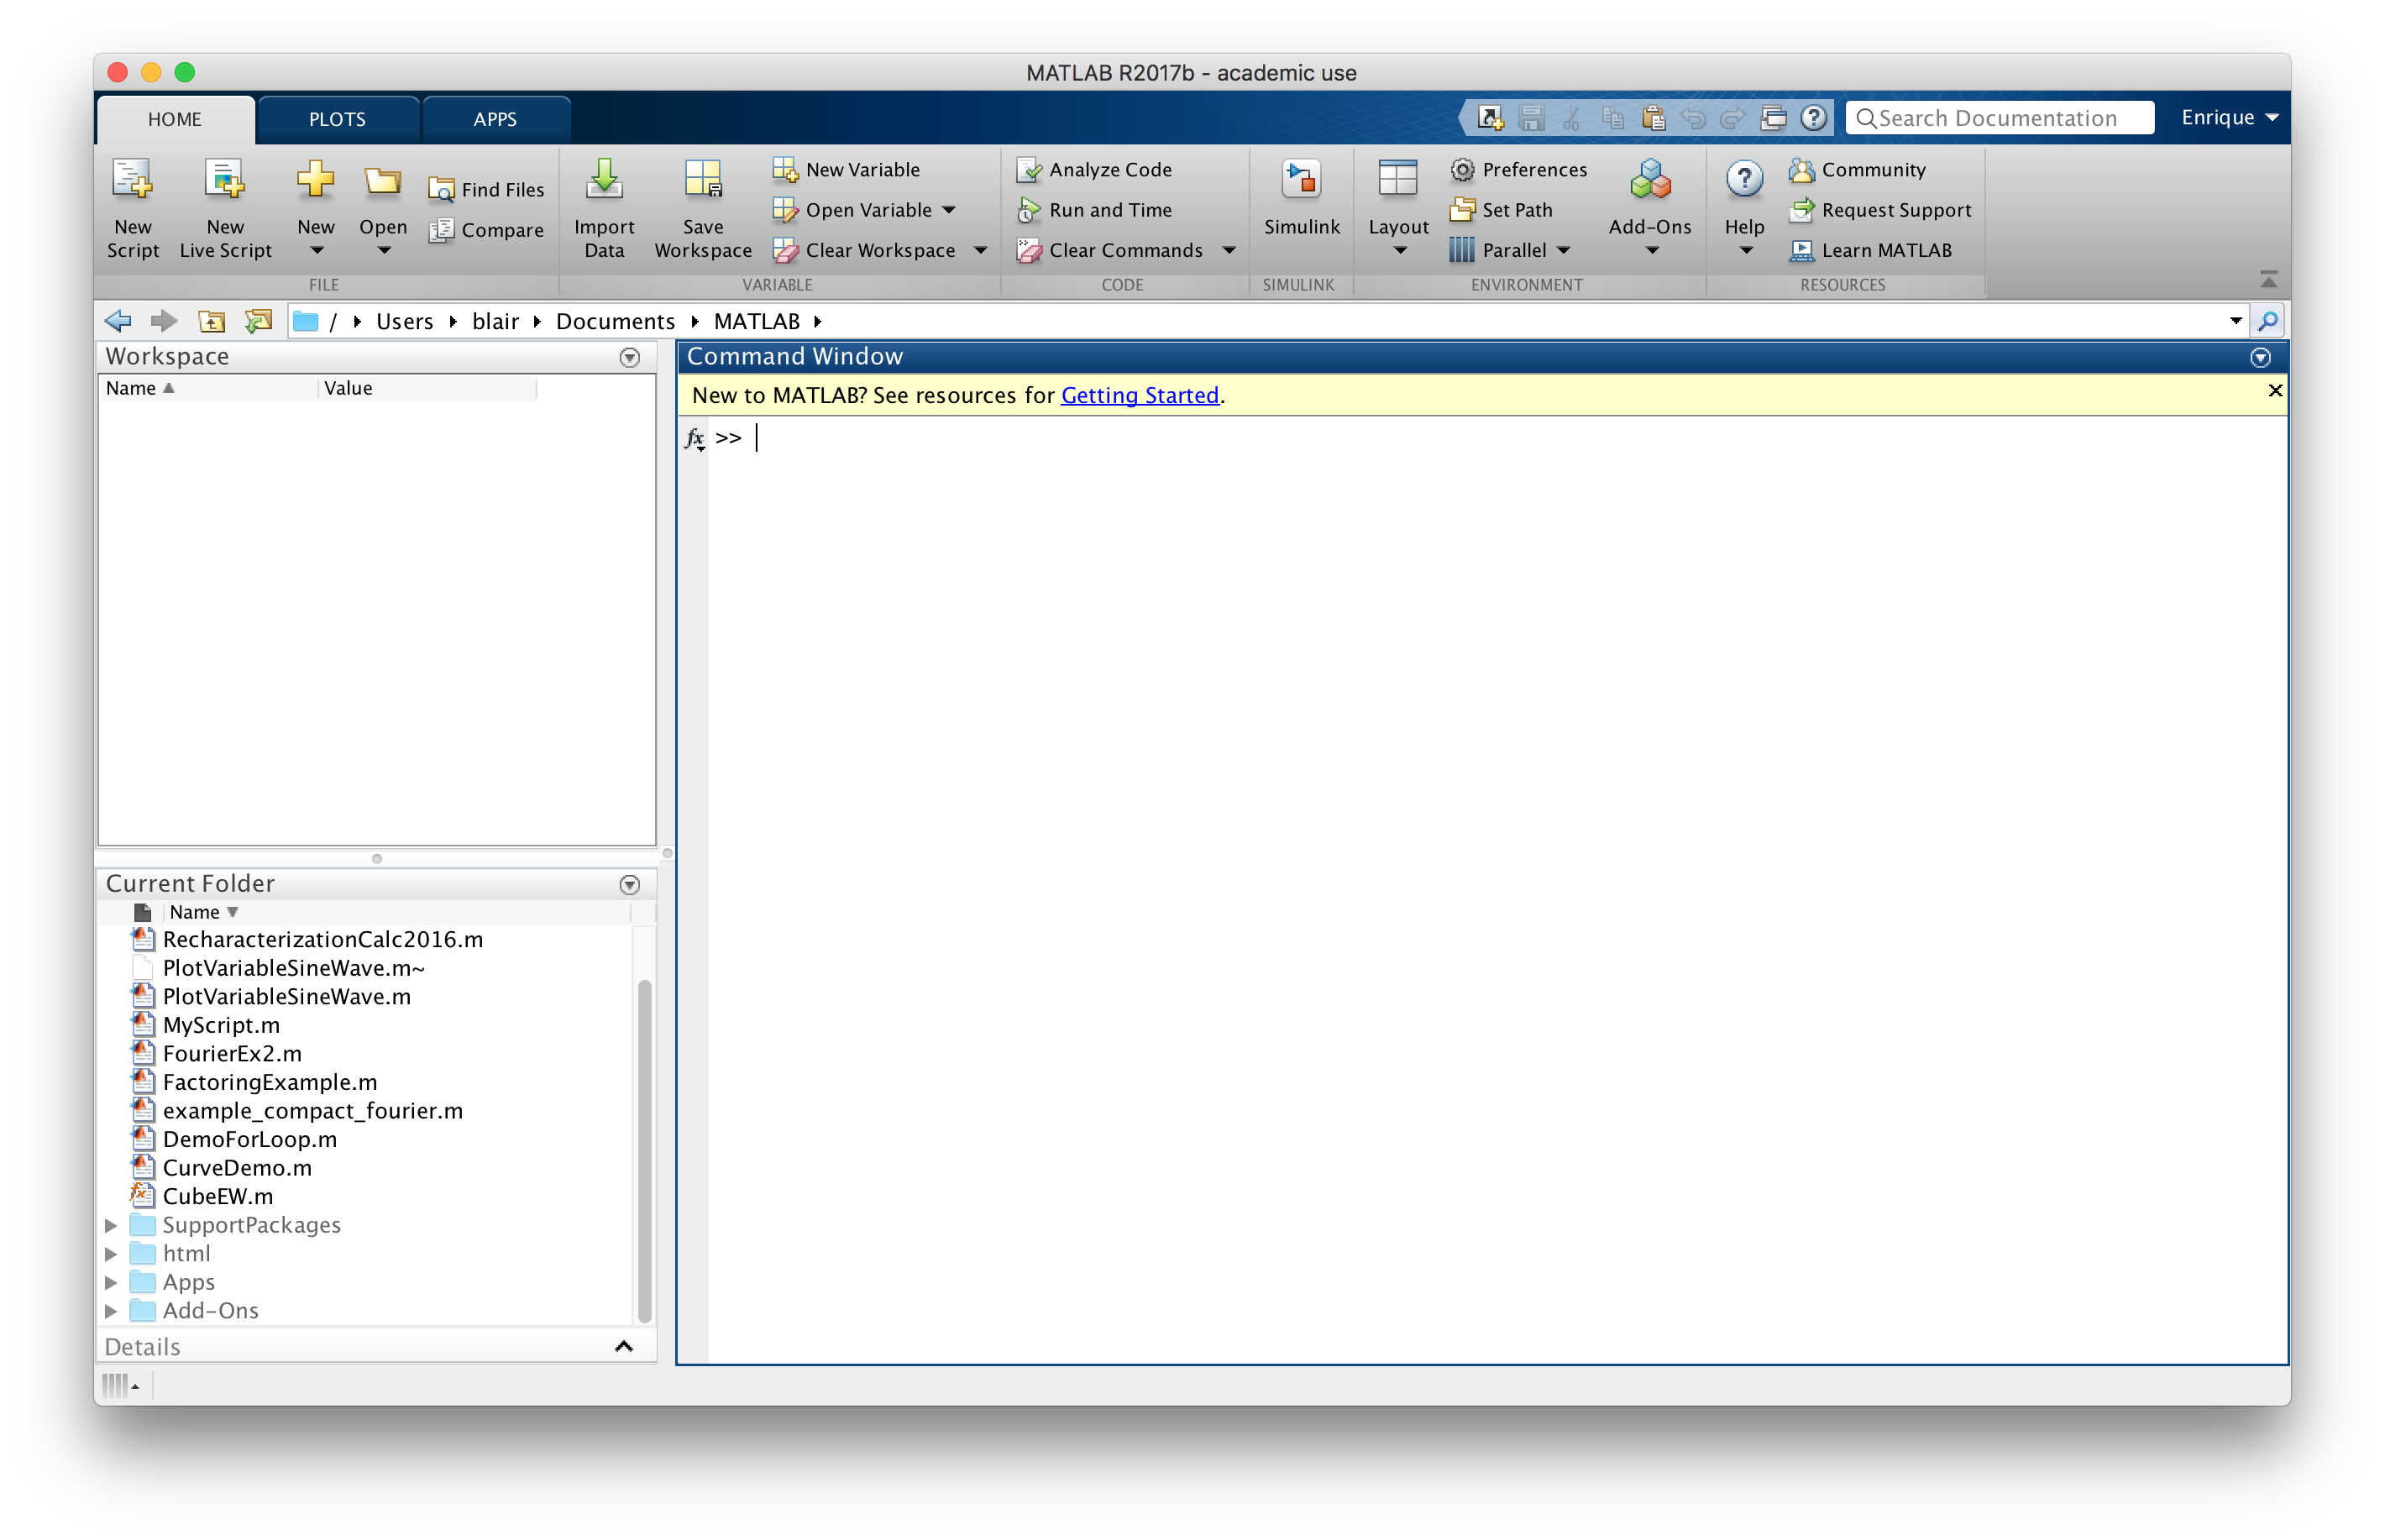
\includegraphics[width=1\textwidth]{graphics/MATLAB_Main_Window.png} 
   \caption{A typical layout for the MATLAB IDE window. It consists of three sub-windows: (1) the Command Window [right]; (2) the Workspace [upper left], and (3) the Current Folder [lower left].}
   \label{fig:MATLAB_IDE}
\end{figure}
% ^^^------------------------------------------------------------^^^

The primary and most commonly-used MATLAB user interface is the MATLAB integrated developing environment (IDE), as shown in Fig. \ref{fig:MATLAB_IDE}. This figure is customizable, but this configuration resembles the default configuration. This configuration has three windows: (1) the Command Window, (2), the Workspace, and (3) the Current Folder. We briefly describe these here:
\begin{enumerate}
\item \textbf{The Command Window}. A user types MATLAB commands at the ``\verb!>>!'' prompt. The Command Window also displays the unsuppressed text output user commands. Commands may be as simple as calculator-like arithmetic to scripts and MATLAB functions.
\item \textbf{The Workspace} lists variables, structures, and objects stored in program memory. The contents of program memory are the result of MATLAB commands and calculations.
\item \textbf{The Current Folder} lists files and subfolders contained within the current folder. The local path to the current folder is also listed in a toolbar near the top. This is important because text files define MATLAB commands, and MATLAB can only use commands associated with files found in the current folder (listed in the Current Folder window) or found within other folders stored in a special \texttt{MATLABPATH} variable. If you attempt to execute a command associated with a file not found in the current folder or in the \texttt{MATLABPATH} folders, then you will get an error in the Command Window that says ``\verb!Undefined function or variable `xxx'!,'' where ``\verb!xxx!'' is replaced by the offending command name.
\end{enumerate}

% ============================================
% ============================================
\subsection{Using MATLAB as a Calculator}
\label{subsect:MATLAB_calculator}
Perhaps the simplest way to use MATLAB is to use it as a calculator by typing mathematical operations in the Command Window. For example, at the MATLAB command prompt ``\verb!>>!'' typing ``\verb!5+6!''  followed by \texttt{RETURN} (\keys{\return}) causes MATLAB to evaluate the sum of 5 and 6. The MATLAB output is shown here:
% vvv------------------------------------------------------------vvv
\begin{lstlisting}[style=Matlab-editor, label={MATLABCalculator01}, caption={A simple addition calculation in MATLAB returns its result.}]
>> 5+6

ans =

    11

>> 
\end{lstlisting}
% ^^^------------------------------------------------------------^^^
In this code listing, line 1 begins with the prompt, ``\verb!>>!'', which is followed by the input typed by the user. MATLAB uses lines 2-6 to report that the answer, 11, is stored in the variable \verb!ans!. The re-emergence of the prompt signifies that MATLAB is ready for a new command.

Another important variation on this command is to assign the result of the mathematical operation to a variable. For example, the following results if we input ``\verb!x=5+6!'':
% vvv------------------------------------------------------------vvv
\begin{lstlisting}[style=Matlab-editor, label={MATLABCalculator02}, caption={The result of the previoius simple addition in MATLAB (see Listing \ref{MATLABCalculator02}) is stored in variable \texttt{x}.}]
>> x=5+6

x =

    11

>> 
\end{lstlisting}
% ^^^------------------------------------------------------------^^^
The command of line 1 is not a statement of equality, but rather an assignment command (we call ``\texttt{=}'' the \textit{assignment operator}). This input instructs MATLAB to evaluate the sum \verb!5+6! and store the result in the variable \texttt{x}. In lines 2-6, MATLAB reports the value that is stored in the variable \texttt{x}. Line 7 again prompts the user for a new command.

Valid MATLAB variable names may contain letters, numbers and underscores. Valid MATLAB variables may not have any spaces, nor can they begin with numbers.

Often, it is desirable to suppress the result of a MATLAB command. This can be accomplished by adding a semicolon \texttt{;} to the command, as follows:
% vvv------------------------------------------------------------vvv
\begin{lstlisting}[style=Matlab-editor, label={MATLABCalculator03}, caption={A semicolon (\texttt{;}) may be used at the end of a MATLAB command to suppress the output.}]
>> x=5+6;
>> 
\end{lstlisting}
% ^^^------------------------------------------------------------^^^
Here, the result of line 1 is suppressed, and the new MATLAB prompt indicates that MATLAB is ready to receive new command. Additionally, the \texttt{;} can be used to divide a single line into several individual commands, as follows:
% vvv------------------------------------------------------------vvv
\begin{lstlisting}[style=Matlab-editor, label={MATLABCalculator04}, caption={The result of a simple addition calculation is saved in the variable \texttt{x}, which is used for a follow-on calculation.}]
>> x=5+6;y=x*2

y =

    22

>>
\end{lstlisting}
% ^^^------------------------------------------------------------^^^
Here, the same command is issued as before, and a second command instructs MATLAB to multiply the value stored in \texttt{x} by 2, and to store the result in a second variable \texttt{y}. Since the second command did not end with a \texttt{;}, its output was not suppressed, and MATLAB reports this result as 22.

\subsubsection{MATLAB Functions}
At this point, we have used the additive and multiplicative binary operators, ``\verb!+!'' and ``\verb!*!'', respectively; as well as the assignment operator ``\verb!=!''. Other valid operators include ``\verb!-!'' (subtraction), ``\verb!/!'' (division), and ``\verb!^!'' (exponentiation). Important functions include \verb!exp()! (the exponential), \verb!sin()! (the sine function), \verb!cos()! (the cosine function) and \verb!tan()! (the tangent function). MATLAB's trigonometric functions accept arguments in radians, but the functions \verb!sind()!, \verb!cosd()!, and \verb!tand()! are degree-input versions of the other trigonometric functions.

MATLAB also recognizes certain predefined constants. We can use ``\texttt{pi}'' to represent the irrational number $\pi$, and ``\texttt{1i}'' is used to represent $i=\sqrt{-1}$. Consider the use of these constants with functions:
% vvv------------------------------------------------------------vvv
\begin{lstlisting}[style=Matlab-editor, label={MATLABCalculator05}, caption={Some examples of pre-defined constants in MATLAB.}]
>> x = cos(pi/2)

x =

   6.1232e-17

>> y = cosd(90)

y =

     0

>> z = exp(1i*pi)

z =

  -1.0000 + 0.0000i
\end{lstlisting}
% ^^^------------------------------------------------------------^^^
Here, lines 1 and 7 evaluate the cosine of $\pi/2$ and $90^\circ$. The results are stored in ``\texttt{x}''  and ``y'', respectively. Note that \texttt{cos(pi/2)} evaluates to a very small number (approximately zero), whereas \texttt{cosd(90)} evaluates to zero.

% ============================================
% ============================================
\subsection{Using MATLAB to Run Scripts}

\subsubsection{Creating a New Script}

It often is helpful to combine many commands in a single file and execute them in sequence as a script. There are several ways to make a new script. One can do any of the following:
\begin{enumerate}
\item Click the ``New Script'' button in the upper right region of the toolbar.
\item Click the ``New Document'' button in the upper right region of the toolbar, and then select ``Script''
\item Press \keys{\cmd+N} on Mac (or \keys{\ctrl+N} on a Windows keyboard)
\item Type \texttt{edit} followed by \keys{\return} in the command window. %Type ``\verb!edit scriptname.m!'' followed by \keys{\return}, where \verb!scriptname.m! is the desired script name with a ``\texttt{.m}'' extension. Note that MATLAB requires valid file names to start with a letter (not a numeral or other special character). Numbers may be included, along with the underscore ``\texttt{\_}'' but special characters and spaces are forbidden. If the script already exists, it will be opened for editing. If it does not exists, you will be asked if you wish to make a new script with the specified name.
\end{enumerate}
Each of these actions opens a new, untitled script for editing in a new Editor window, as seen in Fig.\ \ref{fig:MATLAB_IDE_with_Editor}.

% vvv------------------------------------------------------------vvv
\begin{figure}[htbp] %  figure placement: here, top, bottom, or page
   \centering
   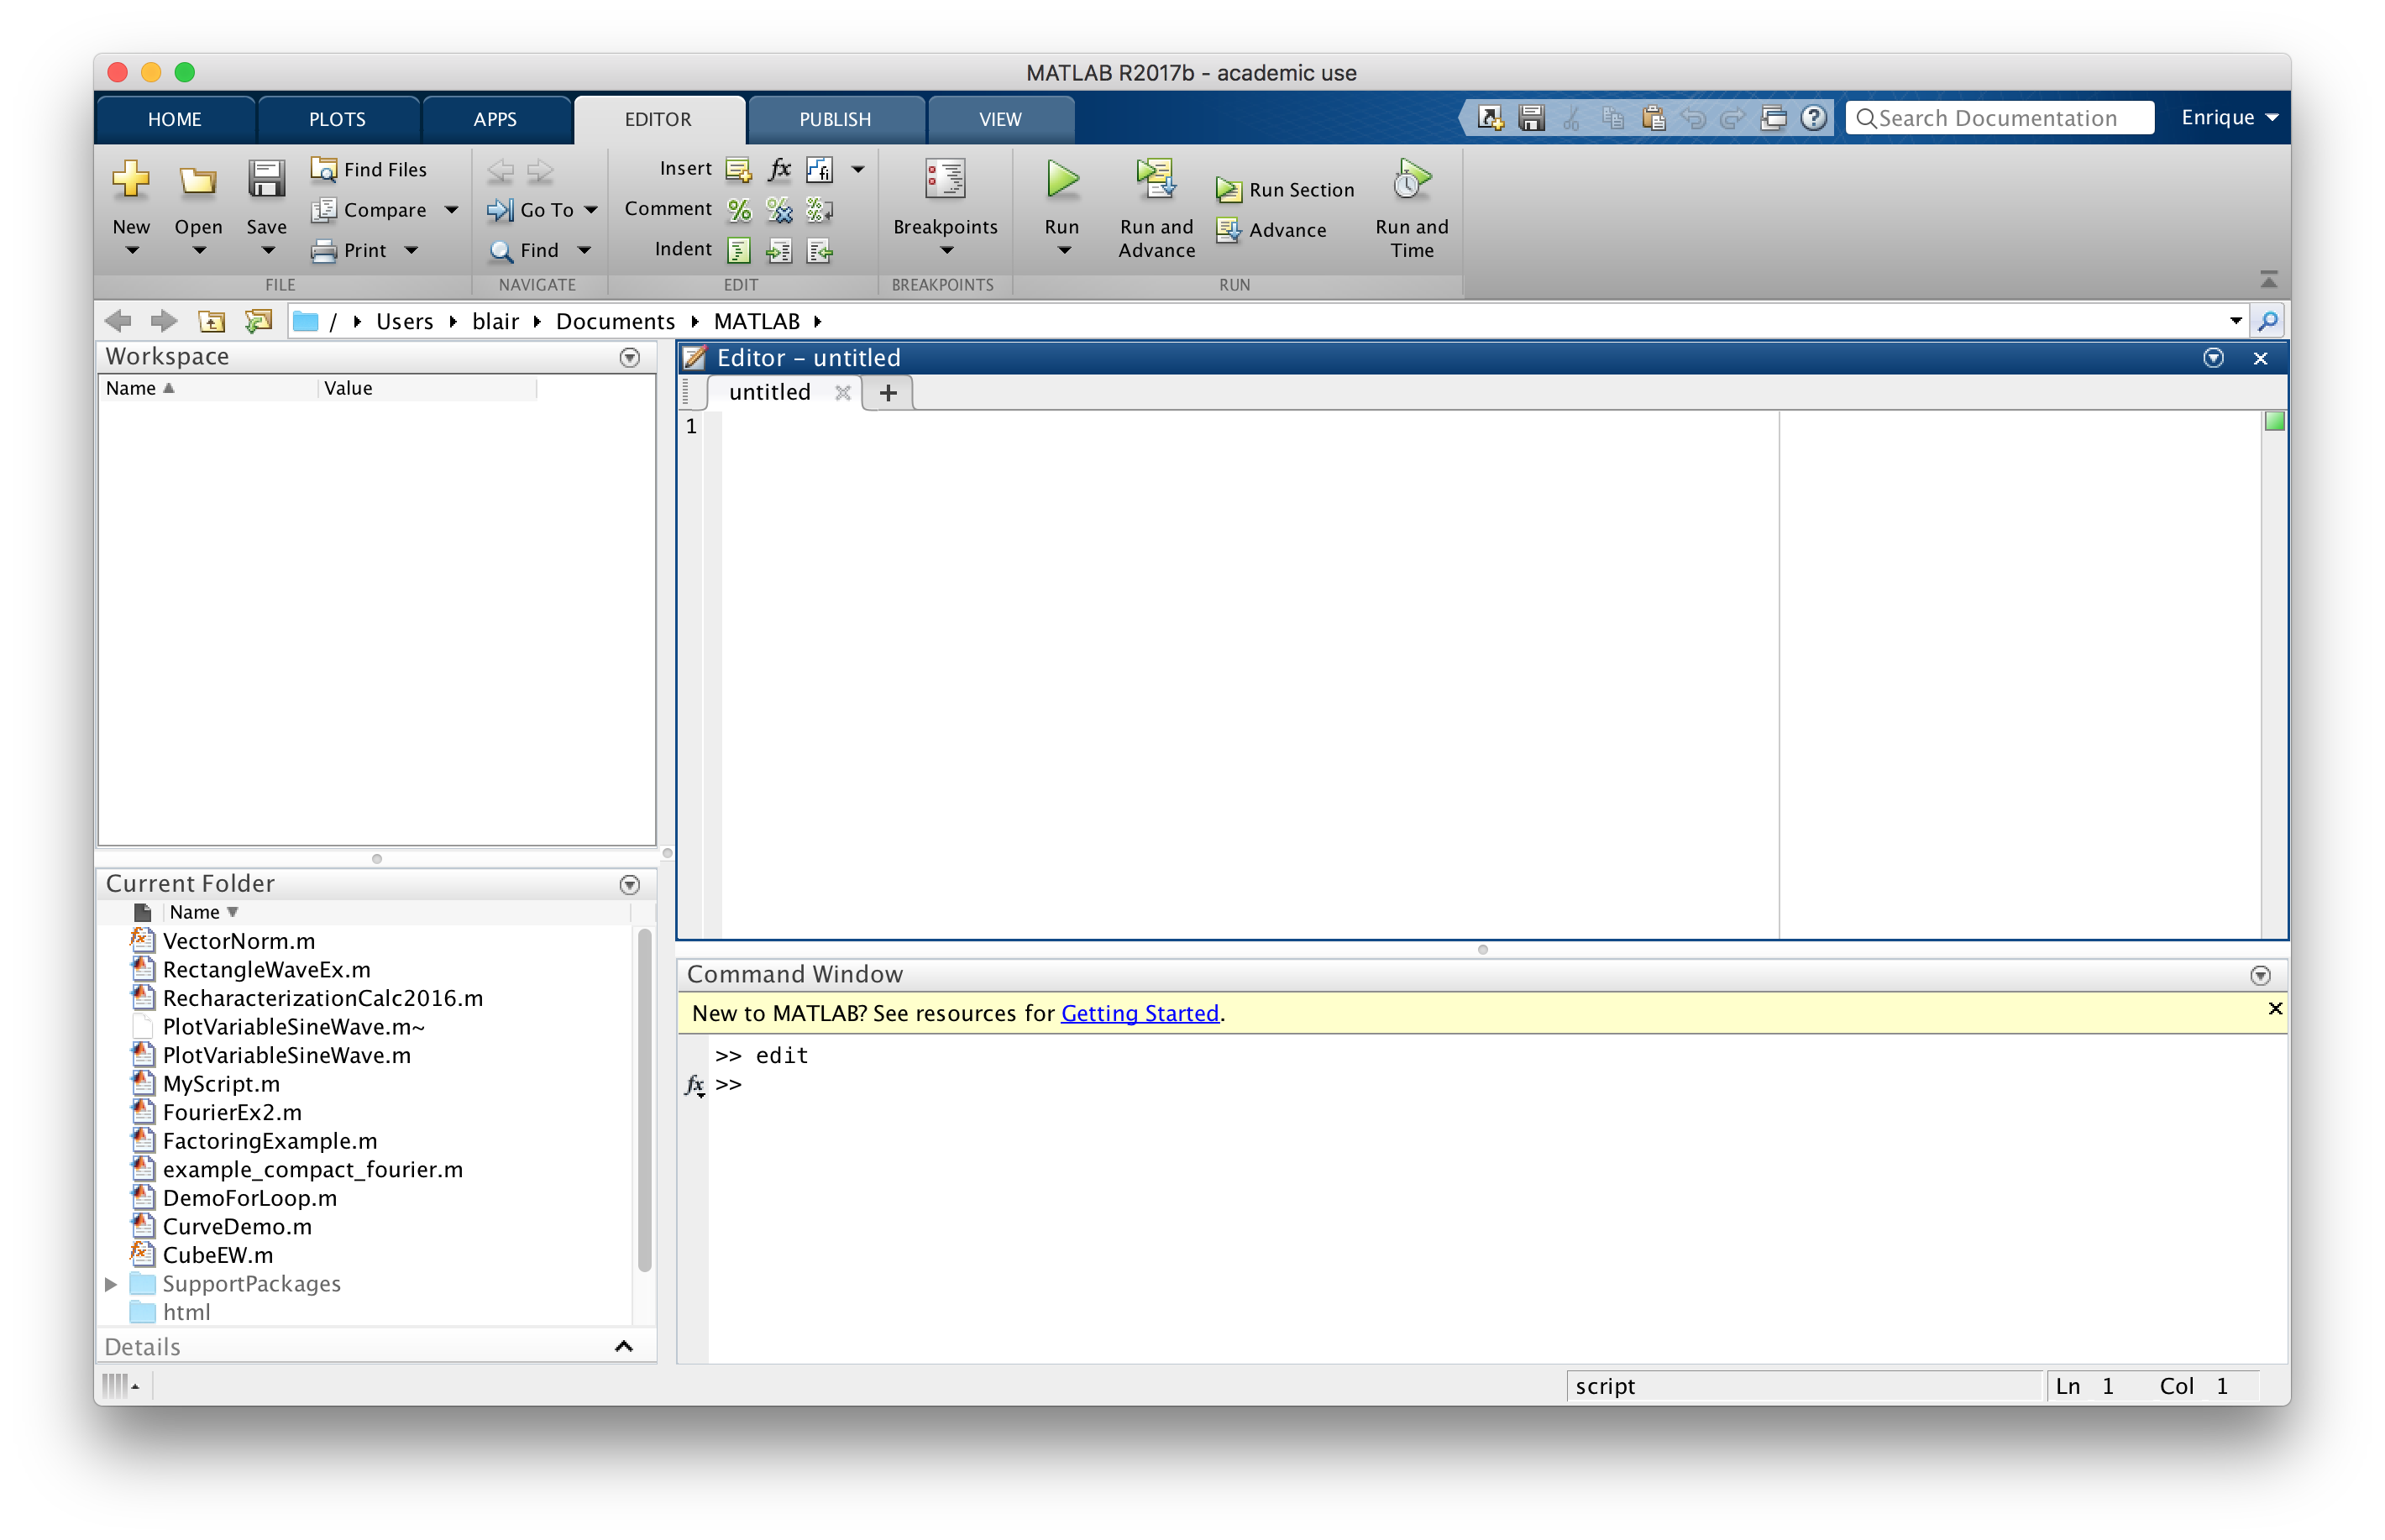
\includegraphics[width=1\textwidth]{graphics/MATLAB_Main_Window_with_Editor.png} 
   \caption{A typical layout for the MATLAB IDE window with an Editor window.}
   \label{fig:MATLAB_IDE_with_Editor}
\end{figure}
% ^^^------------------------------------------------------------^^^



\subsubsection{Writing a Script}
To write the script, write commands in the script just as in section \ref{subsect:MATLAB_calculator}. As before, use ``\texttt{;}'' to suppress output or divide a line into multiple commands. Comments may be added to any line of script by using the ``\texttt{\%}'' symbol. For a given line in the script, any text following a ``\texttt{\%}'' will be ignored and will not be evaluated as a command.

\subsubsection{Executing a Script}
To execute a script, first make sure that the file containing the script is saved in either the current folder or in a folder listed in the \texttt{MATLABPATH} variable. Then, simply type the name of the script exactly (but, without the \texttt{.m} extension) in the command line. Alternately, with the Editor as the active window and the desired script as the active tab within the Editor, click the ``\texttt{Save and Run}'' icon (green right-ward-pointing triangle) in the Editor tab of the toolbar.


% ============================================
% ============================================
% ============================================
\section{Matrix Manipulations}

In MATLAB, all numbers are treated as matrices. The simplest matrix \texttt{A} is an $m \times n$ array of numbers, where $m$ refers to the number of (horizontal) rows and $n$ refers to the number of (vertical) columns in \texttt{A}. Even when we manipulate a single number, MATLAB treats this single number as a $1\times1$ matrix.

Matrices are important in solving systems of equations. They also are useful in MATLAB for storing arrays of numerical data. In this context, matrices may also be called ``storage arrays.''

% ============================================
% ============================================
\subsection{Defining Matrices and Vectors}
A matrix \texttt{A} can be formed by listing each element row by row within a single set of brackets (``\texttt{[}'' and ``\texttt{]}''). Within a row, elements may be separated by white space or by a column, and rows are delimited using semicolons. An example of this is given in the following command and output:
% vvv------------------------------------------------------------vvv
\begin{lstlisting}[style=Matlab-editor, label={MatrixDef01}, caption={A matrix is defined by enumerating its elements and delineating the matrix with brackets (\texttt{`[`} and \texttt{`]`}). Individual elements within a row are separated by a white space, or optionally a comma (\texttt{,}). Rows are separated using a semicolon (\texttt{;}).}]
>> A = [1 2 3 4; 5 6 7 8; 9 10 11 12] % this defines a 3x4 matrix A

A =

     1     2     3     4
     5     6     7     8
     9    10    11    12
\end{lstlisting}
% ^^^------------------------------------------------------------^^^

Alternately, functions such as \texttt{rand()}, \texttt{eye()}, \texttt{zeros()}, \texttt{ones()}, and \texttt{diag()} may be used to create matrices. Consider the following MATLAB script, entitled ``\texttt{MatrixCreation.m}'':
% vvv------------------------------------------------------------vvv
\begin{lstlisting}[style=Matlab-editor, label={MatrixDef02}, caption={Built-in MATLAB functions may be used to create/define matrices.}]
% MatrixCreation.m

m = 3; n = 2; B = rand(m) % defines a pseudorandom m-by-m matrix

C = rand([m,n]) % defines a pseudorandom m-by-n matrix

In = eye(n) % defines an n-by-n identity matrix

Znm = zeros(n, m) % defines an n-by-m matrix of zeros

Omn = ones(m, n) % defines a m-by-n matrix of ones

D = diag([1 2 3 4 5]) % defines a diagonal matrix with the input vector
                      %  on the diagonal
\end{lstlisting}
% ^^^------------------------------------------------------------^^^
Line 3 of \texttt{MatrixCreation.m} defines a $m\times m$ matrix of pseudorandom numbers using the \texttt{rand()} function and stores them in the variable \texttt{B}. Another way to use \texttt{rand()} is to specify a matrix input, where each element of the input matrix specifies a dimension size (the row specification is first, and the column specification comes second). This is done in line 5. In line 7, we use \texttt{eye(n)} to construct a $n\times n$ identity matrix. Line 9 creates a matrix of zeros, and line 11 creates a matrix of ones. Line 13 creates a diagonal matrix. Running \texttt{MatrixCreation.m} results in the following output:
% vvv------------------------------------------------------------vvv
\begin{lstlisting}[style=Matlab-editor, label={MatrixDef02out}, caption={The Command Window output for an invocation of Listing \ref{MatrixDef02}.}]
>> MatrixCreation

B =

    0.4898    0.7094    0.6797
    0.4456    0.7547    0.6551
    0.6463    0.2760    0.1626


C =

    0.1190    0.3404
    0.4984    0.5853
    0.9597    0.2238


In =

     1     0
     0     1


Znm =

     0     0     0
     0     0     0


Omn =

     1     1
     1     1
     1     1


D =

     1     0     0     0     0
     0     2     0     0     0
     0     0     3     0     0
     0     0     0     4     0
     0     0     0     0     5
\end{lstlisting}
% ^^^------------------------------------------------------------^^^

Row vectors are simply $m \times n$ matrices with $m=1$, and column vectors are $m\times n$ matrices with $n=1$. Here are some ways to construct numerical row vectors:
\begin{enumerate}
\item A simple row vector of $n$ integers may be formed by using the syntax ``\verb!k:k+n-1!''. For example, the input \verb!2:5! defines a vector \verb![2 3 4 5]!. This is referred to as a \textit{range} of integers, with unity increment between successive elements. A increment may be specified using ``\verb!min:inc:max!''. For example, the input ``\verb!2:2:10!'' specifies the row vector \verb![2 4 6 8 10]!
\item  A row  vector of floating-point double values may be formed using the syntax ``\verb!min:inc:max!'', where \texttt{min} is the low value, \texttt{max} is the lowest value and the first element in the vector, and each successive element larger than the previous value by \texttt{inc}. No values larger than \texttt{max} are included in the vector.
\item The \texttt{linspace()} command can be used to create row vector of $n$ evenly-spaced points that includes the minimum and maximum values \texttt{min} and \texttt{max} using the syntax ``\verb!linspace(min, max, n)!''
\end{enumerate}


% ============================================
% ============================================
\subsection{Subscripting Matrices}

MATLAB allows us to refer to individual elements of a matrix by using parentheses. If \texttt{A} is a matrix, then \verb!A(row_spec, col_spec)! provides a syntax for subscripting a subset of matrix elements. Here, \verb!row_spec! and \verb!col_spec! are row specifier and column specifier expressions, respectively. The \verb!row_spec! and \verb!col_spec! are also called \textit{indices} (plural of the word, ``index''), and subscripting is also called ``indexing.''

While \verb!row_spec! and \verb!col_spec! must be integers or logical values, there are many ways to specify rows and columns.
\begin{itemize}
\item If \verb!row_spec! and \verb!col_spec! both are single integers, \verb!A(row_spec, col_spec)! specifies a single element of \texttt{A}.
\item A subset of rows or columns may be specified using vectors or ranges. A full row-span or column-span may be achieved by using ``\texttt{:}'' as either the  \verb!row_spec! or \verb!col_spec! expression.
\item When using a vector as a \verb!row_spec! or \verb!col_spec! expression, the \texttt{end} keyword identifies the last valid index for the row or column.
\end{itemize}
Examples of matrix subscripting are given in the code listing of ``\texttt{MatrixSubscripting.m}'':
% vvv------------------------------------------------------------vvv
\begin{lstlisting}[style=Matlab-editor, label={MatrixSubscripting}, caption={Some examples of matrix subscripting, the referencing of a subset of matrix elements.}]
A = [1 2 3 4; 5 6 7 8; 9 10 11 12] % this defines a 3x4 matrix A

A34 = A(3,4) % extract the (3,4) element of A

B = A(2:3,1:3) % extract elements in rows 2-3 and columns 1-3 of A

v = A(:, 2) % extract elements in all rows and colum 2 of A [col. vector]

w = A(3, :) % extract elements row 3 and all columns of A [row vector]

A2end = A(2,end) % extract the last element of row 2

A2endm2_end = A(2, end-2:end) % extract the last three elements of row 2\end{lstlisting}
% ^^^------------------------------------------------------------^^^
When this script is run, the following output results:
% vvv------------------------------------------------------------vvv
\begin{lstlisting}[style=Matlab-editor, label={MatrixSubscriptingOut}, caption={Command Window output for Listing \ref{MatrixSubscripting}.}]
>> MatrixSubscripting

A =

     1     2     3     4
     5     6     7     8
     9    10    11    12


A34 =

    12


B =

     5     6     7
     9    10    11


v =

     2
     6
    10


w =

     9    10    11    12


A2end =

     8


A2endm2_end =

     6     7     8
\end{lstlisting}
% ^^^------------------------------------------------------------^^^

% ============================================
% ============================================
\subsection{Subscripting Matrices and Assignment Statements}

We can assign individual elements or subsets of elements of a matrix by using a subscripted matrix on the left-hand side (LHS) of an assignment statement. Consider the code listing of \texttt{SubscriptedAssignments.m}:
% vvv------------------------------------------------------------vvv
\begin{lstlisting}[style=Matlab-editor, label={MatrixSubscriptingAssign}, caption={Matrix subscripting may be used to assign values to a subset of matrix elements.}]
% SubscriptedAssignments.m

M = zeros(4, 5)

M(2, 5) = 1

M(1:2, 2:3) = 1

M(3:4, 2:4) = rand(2,2)
\end{lstlisting}
% ^^^------------------------------------------------------------^^^
Line 3 defines \texttt{M} as a $4\times 5$ matrix of zeros, with the following result:
% vvv------------------------------------------------------------vvv
\begin{lstlisting}[style=Matlab-editor]
M =

     0     0     0     0     0
     0     0     0     0     0
     0     0     0     0     0
     0     0     0     0     0
\end{lstlisting}
% ^^^------------------------------------------------------------^^^
 Line 5 of \texttt{SubscriptedAssignments.m} stores the value 1 in the $M_{2,5}$, the (2,5) element of \texttt{M}, with this output:
 % vvv------------------------------------------------------------vvv
\begin{lstlisting}[style=Matlab-editor]
M =

     0     0     0     0     0
     0     0     0     0     1
     0     0     0     0     0
     0     0     0     0     0
\end{lstlisting}
% ^^^------------------------------------------------------------^^^
A single scalar value can be assigned to multiple elements of a matrix \texttt{M} simultaneously. As an example of this, line 7 of \texttt{SubscriptedAssignments.m} assigns the single scalar value 1 to a $2\times2$ block of elements in \texttt{M}:
% vvv------------------------------------------------------------vvv
\begin{lstlisting}[style=Matlab-editor]
M =

     0     1     1     0     0
     0     1     1     0     1
     0     0     0     0     0
     0     0     0     0     0
\end{lstlisting}
% ^^^------------------------------------------------------------^^^
In general, however, the LHS and right-hand-side (RHS) of an assignment statement must match in size. Line 9 of \texttt{SubscriptedAssignments.m} demonstrates this: MATLAB throws an error because the target of the assignment on the LHS of line 9 is a $2\times3$ block of elements, but the value on the RHS of line 9 is a $2\times2$ block.
% vvv------------------------------------------------------------vvv
\begin{lstlisting}[style=Matlab-editor]
Subscripted assignment dimension mismatch.

Error in SubscriptedAssignments (line 9)
M(3:4, 2:4) = rand(2,2)
\end{lstlisting}
% ^^^------------------------------------------------------------^^^

% ============================================
% ============================================
\subsection{Concatenation}
Matrices can be combined via concatenation. Horizontal concatenation is the act of creating a larger matrix \texttt{C} from two smaller matrices \texttt{A} and \texttt{B} by setting \texttt{A} and \texttt{B} side-by-side. The syntax for horizontal concatenation is \verb!{C = [A B]!, or equivalently, \verb!{C = [A, B]!. This involves listing the constituent matrices within brackets (\texttt{[} and \texttt{]}) and separating them with either a comma (\texttt{,}) or a white space. An example of this is:
% vvv------------------------------------------------------------vvv
\begin{lstlisting}[style=Matlab-editor, label={MatrixHorizCat}, caption={Matrices may be concatenated horizontally by using brackets and either a comma or a white space to delimit individual elements.}]
>> A = [1 2 3]; B = [4 5 6]; C = [A B]

C =

     1     2     3     4     5     6
\end{lstlisting}
% ^^^------------------------------------------------------------^^^
In the input command line, we define \texttt{A} and \texttt{B} as row vectors, which themselves are horizontal concatenations of three numbers, each. Then, we form \texttt{C} by horizontally concatenating \texttt{A} and \texttt{B}. Horizontal concatenation requires that constituents have the same number of rows. Concatenation can be thought of as making a matrix of matrices.

Vertical concatenation is accomplished in the same was as horizontal concatenation, except that constituent matrices must have the same number of columns, and constituent matrices must be separated by a semicolon ('\texttt{;}'). The following listing forms the matrix \texttt{D} by vertically concatenates \texttt{A} and \texttt{B}:
% vvv------------------------------------------------------------vvv
\begin{lstlisting}[style=Matlab-editor, label={MatrixVertCat}, caption={Matrices may be concatenated vertically by using brackets and either a semicolon to delimit individual elements.}]
>> D = [A; B]

D =

     1     2     3
     4     5     6
\end{lstlisting}
% ^^^------------------------------------------------------------^^^

 
% ============================================
% ============================================
\subsection{Single-subscripting}
Matrices also may be subscripted with a single index, instead of using both \texttt{row\_spec} and \texttt{col\_spec} specifiers. For an $m\times n$ matrix \texttt{A}, the element \texttt{A(1)} is the $A_{1,1}$ element in the upper left. MATLAB is known as a \textit{column-major} language, in which elements are counted down the columns. Thus, \texttt{A(2)} refers to $A_{2,1}$, which is the element immediately below $A_{1,1}$ in column 1; and \texttt{A(3)} refers to $A_{2,1}$. When the end of the column is reached, the counting continues at the top of the next column.

A simple application of this is the subscripting of a vector \texttt{A}. The expression \texttt{A(k)} refers to the $k$-th element of \texttt{A}, regardless of whether \texttt{A} is a row vector or a column vector. 
 % ============================================
% ============================================
\exmp{Example} \label{Exmp:Cosines}
Define a row vector \texttt{t} that includes $n_t = 75$ time points from $t=0$ to $t=1$ (inclusive). Then, define a matrix \texttt{fn} to represent $f_n (t) = \cos (2\pi n t)$ over the interval $t\in [0, 1]$ for $n \in \{1, 2, 3, 4\}$.

\noindent \underline{Solution}
The solution is given in the code listing of \texttt{Sinusoids.m}.
% vvv------------------------------------------------------------vvv
\begin{lstlisting}[style=Matlab-editor]
% Sinusoids.m
%
% By E.P. Blair
% Baylor University
%

nt = 75; % number of time points
t = linspace(0, 1, nt); % [s] define a time vector

fn = zeros(4, nt); % Define a storage array to hold fn calculations
                   % The n^th row of fn stores fn = cos(2*pi*n*t)
      
% calculate fn and store fn for each value of n in the n^th row
fn(1,:) = cos(2*pi*t); % n = 1
fn(2,:) = cos(2*pi*2*t); % n = 2
fn(3,:) = cos(2*pi*3*t); % n = 3
fn(4,:) = cos(2*pi*4*t); % n = 4
\end{lstlisting}
% ^^^------------------------------------------------------------^^^

So far, we have discussed MATLAB numerical data. Numbers in MATLAB are double-precision floating-point values, or simply \verb!double!. MATLAB uses 8 bytes of memory to store each one. When storing complex numbers, MATLAB uses two doubles for each individual number: one for the real part, and one for the complex part. 

% ============================================
% ============================================
\subsection{The \texttt{char} Data Type and Strings}

Now we consider data of type \verb!char!, which is short for ``character.'' MATLAB \texttt{char}s store individual letters (uppercase [\texttt{A}-\texttt{Z}] or lowercase [\texttt{a}-\texttt{z}]), numerals (\texttt{0}-\texttt{9}), and special characters (\verb!~!, \verb!!!, \verb!@!,  \verb!#!, etc.). Data of type \verb!char! may be stored in a variable using an assignment statement. In MATLAB, we identify a character using a pair of single quotes, as follows in this MATLAB command line input and resulting output:
% vvv------------------------------------------------------------vvv
\begin{lstlisting}[style=Matlab-editor, caption={Simple definition of \texttt{char} variables in the Command Window.}]
>> x = '1'

x =

    '1'

>> y = 1

y =

     1

>> 
\end{lstlisting}
% ^^^------------------------------------------------------------^^^
Here, we have stored the \texttt{char} data \texttt{'1'} in the variable \texttt{x} (line 1, with output on line 3). We contrast this with the case where we store numerical (\texttt{double} data (the value 1) in the variable \texttt{y} (line 7, with output on line 9). The \texttt{char} data \verb!'1'! is distinguished from the \texttt{double} data 1 by the single quotes.


\subsubsection{Strings}
A string is simply an array of \texttt{char}s. A string may be defined using the following syntax:
% vvv------------------------------------------------------------vvv
\begin{lstlisting}[style=Matlab-editor, caption={Simple definition of a \texttt{char} string and its output.}]
>> x = 'hello world'

x =

    'hello world'
\end{lstlisting}
% ^^^------------------------------------------------------------^^^
It is most typical to work with strings as row vectors, but column vectors and general matrices also may be constructed. Matrix concatenations are available for strings:
% vvv------------------------------------------------------------vvv
\begin{lstlisting}[style=Matlab-editor, caption={Horizontal and vertical string concatenations.}]
>> x = 'cat'; y = 'dog'; z = [x y]

z =

    'catdog'
>> w = [x; y]

w =

  2�3 char array

    'cat'
    'dog'
\end{lstlisting}
% ^^^------------------------------------------------------------^^^



% !TEX root = MATLAB_Introduction_Blair.tex

% ============================================
% ============================================
\section{Basic Visualization}
The code of Example \ref{Exmp:Cosines} executes, but we have not yet shown a way to visualize the result to verify the calculation. To do this, we introduce basic plotting.

A very useful command is the \texttt{plot()} command, which can make line graphs. One very general syntax for \texttt{plot()} is of the form \verb!plot(X1, Y1, X2,Y2, X3, Y3,...)!, where \texttt{Xk} and \texttt{Yk} are vectors of equal length storing $x$-data and $y$-data, respectively, with $k \in \{1, 2, 3, \ldots\}$. To adapt this syntax to the code of Example \ref{Exmp:Cosines}, we use \texttt{t} in the place of each of \texttt{X1}, \texttt{X2}, \texttt{X3}, and \texttt{X4}. Also, we use \texttt{fn(:,}$k$\texttt{)} in place of \verb!Y!$k$.
% vvv------------------------------------------------------------vvv
\begin{lstlisting}[style=Matlab-editor]
plot( t, fn(:,1), t, fn(:,2), t, fn(:,3), t, fn(:,4) );
\end{lstlisting}
% ^^^------------------------------------------------------------^^^

In the case of Example \ref{Exmp:Cosines}, however, \texttt{X1}, \texttt{X2}, \texttt{X3}, and \texttt{X4} are indentically equal to the \texttt{t} vector; additionally, all the sets of $y$-data are stored as rows of the \texttt{fn} matrix. In this case, we can use the simpler syntax
% vvv------------------------------------------------------------vvv
\begin{lstlisting}[style=Matlab-editor]
plot( t, fn);
\end{lstlisting}
% ^^^------------------------------------------------------------^^^
The result of this listing or the prior one are equivalent. We append this visualization code to the end of \texttt{Sinusoids.m}, resulting in a new script, \verb!Sinusoids_v01.m!:
% vvv------------------------------------------------------------vvv
\begin{lstlisting}[style=Matlab-editor]
% Sinusoids_v01.m
% 
% This is the same as Sinusoids.m, but adds visualization.
%
% By E.P. Blair
% Baylor University
%

nt = 75; % number of time points
t = linspace(0, 1, nt); % [s] define a time vector

fn = zeros(4, nt); % Define a storage array to hold fn calculations
                   % The n^th row of fn stores fn = cos(2*pi*n*t)
      
% calculate fn and store fn for each value of n in the n^th row
fn(1,:) = cos(2*pi*t); % n = 1
fn(2,:) = cos(2*pi*2*t); % n = 2
fn(3,:) = cos(2*pi*3*t); % n = 3
fn(4,:) = cos(2*pi*4*t); % n = 4

plot(t, fn);
\end{lstlisting}
% ^^^------------------------------------------------------------^^^
The result of this listing is shown in Fig.\ \ref{fig:Sinusoids_v01}. Here, we see the set of sinusoids represented by $f_n (t)$ plotted for $n \in \{1, 2, 3, 4\}$. However, this plot may be improved in several ways:
\begin{enumerate}
\item The sinusoids are not smooth: they look as though they are only approximated using straight line segments. plot requires labels that help assign meaning to the data.
\item This plot requires labels that help assign meaning to the data.
\begin{enumerate}
\item The $x$-axis and $y$-axis both need \textit{labels}.
\item There should be a \textit{legend} to disambiguate the various lines in the plot.
\end{enumerate}

\item A grid may be added to assist in reading the graph.
\item The data lines themselves may be thickened for improved visibility.
\end{enumerate}

These changes can be achieved by using \verb!Sinusoids_v02.m!:
% vvv------------------------------------------------------------vvv
\begin{lstlisting}[style=Matlab-editor,label=lstSinusoids_v02, caption={Listing of the \texttt{Sinusoids\_v02.m} script.}]
% Sinusoids_v02.m
% 
% This is the same as Sinusoids_v01.m, but improves the visualization.
%
% By E.P. Blair
% Baylor University
%

nt = 150; % number of time points
t = linspace(0, 1, nt); % [s] define a time vector

fn = zeros(4, nt); % Define a storage array to hold fn calculations
                   % The n^th row of fn stores fn = cos(2*pi*n*t)
      
% calculate fn and store fn for each value of n in the n^th row
fn(1,:) = cos(2*pi*t); % n = 1
fn(2,:) = cos(2*pi*2*t); % n = 2
fn(3,:) = cos(2*pi*3*t); % n = 3
fn(4,:) = cos(2*pi*4*t); % n = 4

plot(t, fn, 'LineWidth', 2); % thickens the data lines
grid on; % makes the grid visible
set(gca, 'FontSize', 18, 'FontName', 'Times');
xlabel('$t$ (s)', 'Interpreter', 'latex')
ylabel('$f_n(t)$', 'Interpreter', 'latex')
sine_lgnd = legend('$f_1$', '$f_2$', '$f_3$', '$f_4$')
sine_lgnd.Interpreter = 'latex';
\end{lstlisting}
% ^^^------------------------------------------------------------^^^
In this listing, line 9 increases the number of data points so that the plots become smoother. Line 21 uses optional inputs to \verb!plot()! in a \textbf{property-value} pair, specifically, \verb!`LineWidth', 2! to increase the weight of the lines drawn. Line 22 turns the grid on. Line 23 uses \texttt{gca} (get current axes) to get a handle to the current axes. This handle, then is used within the \texttt{set()} function to modify properties of the current axes using property-value pairs. Specifically, we set the font size to 18, and the font name to \texttt{'Times'}. Lines 24 and 25 generate the labels for the $x$- and $y$-axes. Notice here that the first argument to \texttt{xlabel()} or \texttt{ylabel()} is the desired string, and that some of the string is enclosed in dollar signs (\verb!$!). These tell MATLAB to use \LaTeX \, syntax to mathematically typeset the expression or equation contained inside the paired \verb!$! signs. In order for this to work, we can to use the property value pair \verb!'Interpreter', 'latex'! to indicate that MATLAB needs to perform some \LaTeX \, typesetting. In line 26, we use the \texttt{legend()} command to create the legend, and we save the handle by which we reference the legend object by assigning it to a variable, \verb!sine_lgnd!. The inputs to \texttt{legend()} are character strings, and again, we used \LaTeX \, formatting. In order for this to work, we set the \texttt{Interpreter} property of \verb!sine_lgnd!  to \verb!'latex'!. The result of this code is shown in Fig.\ \ref{fig:Sinusoids_v02}.

\begin{figure}[htbp] %  figure placement: here, top, bottom, or page
   \centering
   \subfigure[Output for listing of \texttt{Sinusoids\_v01.m}.]{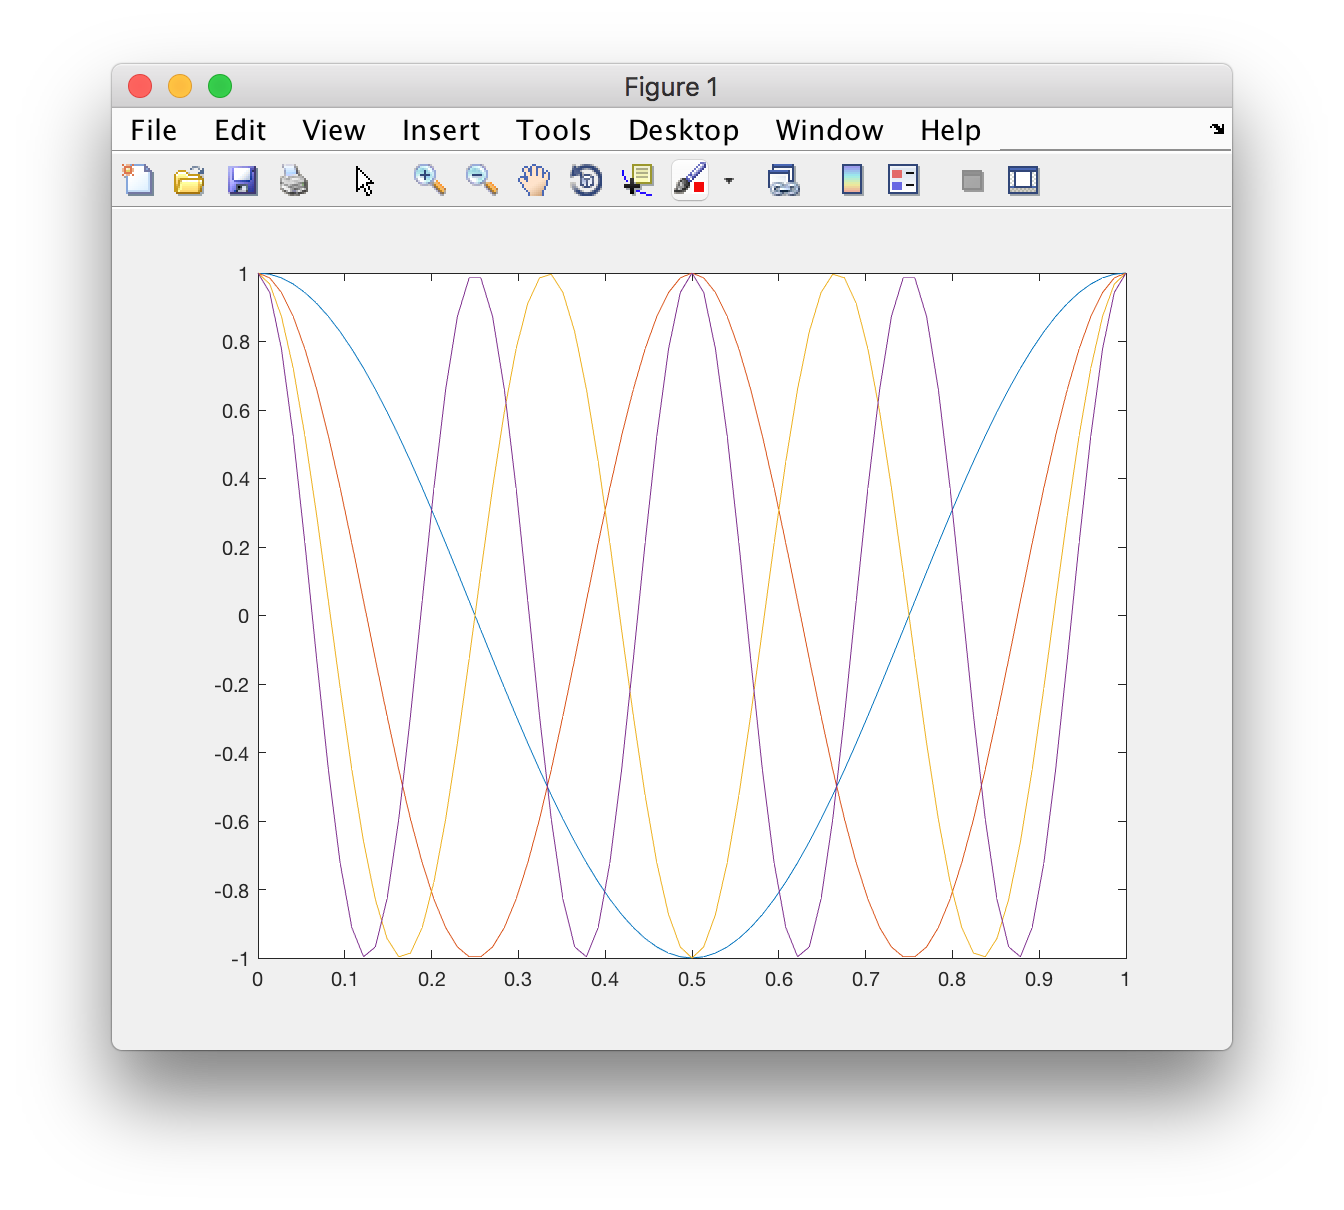
\includegraphics[width=0.485\textwidth]{graphics/Fig_Sinusoids_v01.png} \label{fig:Sinusoids_v01}
   }
   \subfigure[Output for listing of \texttt{Sinusoids\_v02.m}.]{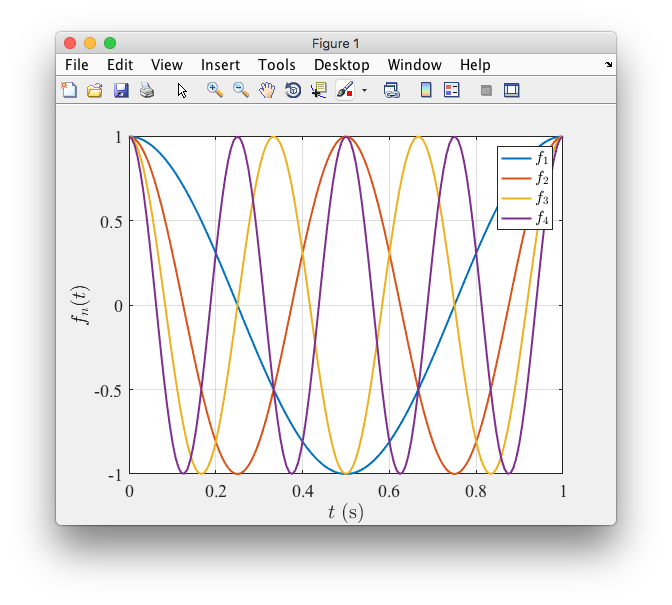
\includegraphics[width=0.485\textwidth]{graphics/Fig_Sinusoids_v02.png} \label{fig:Sinusoids_v02}
   }
   \caption{Plots of the sinusoids calculated in Example \ref{Exmp:Cosines}.}
   \label{fig:Sinusoids_output}
\end{figure}


% !TEX root = MATLAB_Introduction_Blair.tex
\section{\texttt{for} Loops}

\subsection{Some Useful Non-numerical Functions}

We briefly introduce some MATLAB functions that will help us illustrate a \texttt{for} loop.

\subsubsection{The \texttt{disp()} Function}
MATLAB comes with some helpful non-numerical functions. For example, the \texttt{disp()} function prints a string to the output. Here are two example uses of the \texttt{disp()} function:
% vvv------------------------------------------------------------vvv
\begin{lstlisting}[style=Matlab-editor]
>> disp('hello world')
hello world
>> someStr = 'hello world'; disp(someStr)
hello world
\end{lstlisting}
% ^^^------------------------------------------------------------^^^
In the first example (line 1), we provide the string \verb!'hello world'! within the input to \texttt{disp()} itself. In the second example (line 3), we first store \verb!'hello world'! in the variable \texttt{someStr}, and then we pass \texttt{someStr} to the \texttt{disp()} function. In both cases, the output is the same.

\subsubsection{The \texttt{num2str()} Function}
If we wish to print a number, we first convert it to a string using the \texttt{num2str()} function.
% vvv------------------------------------------------------------vvv
\begin{lstlisting}[style=Matlab-editor]
>> b = num2str('42')

b =

    '42'

>> k = 27; disp(['k = ', num2str(k)])
k = 27
>> 
\end{lstlisting}
% ^^^------------------------------------------------------------^^^
In this example, we convert the number 42 to the string \texttt{'42'}, and store it in the variable \texttt{b} (line 1). Then, in line 7, we assign the number 27 to the variable \texttt{k}. We append the string representing the value of \texttt{k} onto the string \verb!'k = '!, and we pass this to \texttt{disp()}, with the result of line 8.

% ==================================================================
% ==================================================================
\subsection{\texttt{for} Loops}
% ==================================================================
% ==================================================================

A \texttt{for} loop has the following syntax:
% vvv------------------------------------------------------------vvv
\begin{lstlisting}[style=Matlab-editor]
for variable = expr, statement, ..., statement END
\end{lstlisting}
% ^^^------------------------------------------------------------^^^
It begins with the key word \texttt{for} and ends with the key word \texttt{end}. The placeholder \texttt{expr} usually is an expression that defines or references a matrix or an array. The placeholder \texttt{statement, ..., statement} represents the body of the for loop. The body is executed as many times as dictated by the instruction \texttt{for variable = expr}. In each iteration, the variable \texttt{variable} \textemdash known as the \texttt{for}-loop variable \textemdash references some subset of \texttt{expr} and may be manipulated within the body.

A more typical and readable format for a \texttt{for} loop is as follows:
% vvv------------------------------------------------------------vvv
\begin{lstlisting}[style=Matlab-editor]
for variable = expr
   statement
   ...
   statement
end
\end{lstlisting}
% ^^^------------------------------------------------------------^^^
This produces the same result as the previous listing, but the structure of the loop and the body are (desirably) more clearly visible to a reader.

If \verb!expr! is an array, then the \texttt{for} loop iterates once for each element of \verb!expr!. In the $k$-th iteration of the the loop, \verb!variable! is accessible and takes the value of the $k$-th element of \verb!expr!.

Consider the following listing, in which we define \verb!v! as a $1\times 5$ array of type \texttt{double} (\verb!v = [1 2 3 4 5]!), and we make MATLAB display each element, one at a time:
% vvv------------------------------------------------------------vvv
% basicForLoop.m
\begin{lstlisting}[style=Matlab-editor, label={basicForLoop_listing}]
% basicForLoop.m
% Demonstrates a basic for loop

v = 1:5;
for k = v
   disp(['The value of k is ', num2str(k)]);
end
\end{lstlisting}
% ^^^------------------------------------------------------------^^^
For each loop iteration, the value of \verb!k! is displayed, and \verb!k! takes the value of a different element of \verb!v! in each iteration. 
% vvv------------------------------------------------------------vvv
% basicForLoop.m
\begin{lstlisting}[style=Matlab-editor, label={basicForLoop_listing}]
>> basicForLoop
The value of k is 1
The value of k is 2
The value of k is 3
The value of k is 4
The value of k is 5
\end{lstlisting}
% ^^^------------------------------------------------------------^^^

In the following listing, \verb!basicForLoop_v01.m! a modified loop vector \texttt{v} starts with \verb!v_idx = v(1)! (starting at five), and each successive \texttt{v(k)} is two less than the previous value. This continues as long as  \verb!v_idx! is greater than equal to the far end of \texttt{v}.
The code of \verb!basicForLoop_v01.m! is as follows:
% vvv------------------------------------------------------------vvv
% basicForLoop.m
\begin{lstlisting}[style=Matlab-editor, label={basicForLoop_v01_listing}]
% basicForLoop_v01.m
% Demonstrates a basic for loop

v = 5:-2:-12;
for k = v
   disp(['The value of k is ', num2str(k)]);
end
\end{lstlisting}
% ^^^------------------------------------------------------------^^^
This yields the result
% vvv------------------------------------------------------------vvv
% basicForLoop.m
\begin{lstlisting}[style=Matlab-editor, label={basicForLoop_v01_listing}]
>> basicForLoop_v01
The value of k is 5
The value of k is 3
The value of k is 1
The value of k is -1
The value of k is -3
The value of k is -5
The value of k is -7
The value of k is -9
The value of k is -11
\end{lstlisting}
% ^^^------------------------------------------------------------^^^

\subsubsection{\texttt{for}-loop Automation}
The listing \verb!Sinusoids_v02.m! (Listing \ref{lstSinusoids_v02}) may be written elegantly using a \texttt{for} loop. This is accomplished in \verb!Sinusoids_v03.m!:
% vvv------------------------------------------------------------vvv
\begin{lstlisting}[style=Matlab-editor, label={Sinusoids_v03_listing}, caption={The functionality of \texttt{Sinusoids\_v02.m} is duplicated here, this time using a \texttt{for} loop.}]
% Sinusoids_v03.m
% 
% This is the same as Sinusoids_v02.m, but uses a for loop.
%
% By E.P. Blair
% Baylor University
%

N = 4; % number of sinusoids (maximum value of N)
nt = 150; % number of time points
t = linspace(0, 1, nt); % [s] define a time vector

fn = zeros(4, nt); % Define a storage array to hold fn calculations
                   % The n^th row of fn stores fn = cos(2*pi*n*t)
      
% calculate fn and store fn for each value of n in the n^th row
for n_idx = 1:N
    fn(n_idx,:) = cos(2*pi*n_idx*t);
end

plot(t, fn, 'LineWidth', 2); % thickens the data lines
grid on; % makes the grid visible
set(gca, 'FontSize', 18, 'FontName', 'Times');
xlabel('$t$ (s)', 'Interpreter', 'latex')
ylabel('$f_n(t)$', 'Interpreter', 'latex')
sine_lgnd = legend('$f_1$', '$f_2$', '$f_3$', '$f_4$')
sine_lgnd.Interpreter = 'latex';
\end{lstlisting}
% ^^^------------------------------------------------------------^^^
Lines 15-19 of Listing \ref{lstSinusoids_v02} map to Lines  17-19 here. While the gain is not impressive, it can be helpful, especially if we must repeat a task tens, hundreds, or thousands of times. It makes code much easier to read when \texttt{for} loops are used.

Some best practices when using \texttt{for} loops include the use of a meaningful \texttt{for}-loop variable, and using indentation within the loop to distinguish the body from the beginning and end, as well as from code outside of the loop. Finally, if we do not necessarily know how long a vector is, and we wish to operate on each element, we can use the \texttt(length()) function:
% vvv------------------------------------------------------------vvv
\begin{lstlisting}[style=Matlab-editor, label={Sinusoids_v03_listing}, caption={The \texttt{length()} function can be used to determine the number of times a \texttt{for} loop should iterate to operate on each value of the vector \texttt{x}.}]
...
for x_idx = 1:length(x)
   statements
end
\end{lstlisting}
% ^^^------------------------------------------------------------^^^


\subsubsection{\texttt{for} Loops Aren't Always the Best Tool}
\texttt{for} loops have their place, but they are not necessarily the best tool for certain tasks. For example, if we define \texttt{x} using \verb!x = 1:7!, we could use a \texttt{for} loop to calculate the elements of \texttt{y}, for which \verb!y(k) = x(k)^2!, but it will be faster and more elegant if we use the \verb!.^! (element-wise exponentiation) operator. This is illustrated in Listing \ref{bad_for_usage}, below.
% vvv------------------------------------------------------------vvv
\begin{lstlisting}[style=Matlab-editor, label={bad_for_usage}, caption={Element-wise operations may be faster and more elegant than using a \texttt{for} loop. Here, we use a \texttt{for} loop to square every element of \texttt{x} and store the result in \texttt{y} (lines 5-7). Alternately, we use an element-wise exponentiation to square each element of \texttt{x} and save the results in \texttt{y2}. The element-wise exponentiation is faster, more efficient, clearer, and more concise than the \texttt{for}-loop approach.}]
% poor_for_usage.m

x = 1:7;
y = zeros(1, length(x)); % pre-define a storage vector for the result
for x_idx = 1:length(x)
    y(x_idx) = x(x_idx)^2;
end
y

y2 = x.^2
\end{lstlisting}
% ^^^------------------------------------------------------------^^^
This produces the following output
% vvv------------------------------------------------------------vvv
\begin{lstlisting}[style=Matlab-editor, label={bad_for_usage_output}, caption={The output of Listing \ref{bad_for_usage} shows a case where an element-wise operation yields the same result as a \texttt{for}-loop execution.}]
>> poor_for_usage

y =

     1     4     9    16    25    36    49


y2 =

     1     4     9    16    25    36    49
\end{lstlisting}
% ^^^------------------------------------------------------------^^^

% !TEX root = MATLAB_Introduction_Blair.tex

\section{Extending MATLAB: Writing User-defined Functions}

A powerful way to extend a programming language is to write functions. A well-written function serves as a robust piece of code that can be seamlessly and simply used repeatedly and in different contexts with an invocation to the function. A simple function invocation can belie very complex inner workings, which a user need not reprogram or copy and paste. Complex software can be built in a clear and concise way from robust, rigorously-tested functions.

A function performs a specific task. It may receive input parameters or \textit{input arguments} that determine the results of the function. Some output values\textemdash called \textit{output arguments} \textemdash may be returned by the function.

% ============================================================
\subsection{Writing Functions}
% ============================================================
A MATLAB function is typically defined in a text file with the extension \texttt{*.m}. Functions also may be defined within a script, but in this case, they are only accessible within that script and must appear at the bottom of the script. The former method provides more flexibility and power than the latter, so we prefer to give each function its own appropriately-named \texttt{*.m} file. Here are some salient features of such a function definition file.

\begin{enumerate}
\item The name of the \texttt{*.m} file must match the function name exactly (MATLAB is case-sensitive).
\item The file begins with the keyword \texttt{function}, followed by the name of the function. This first line of the function is called the \textit{header}, and it specifies how the user interacts with the function. The syntax of the function header (with end) is given below:
% vvv------------------------------------------------------------vvv
\begin{lstlisting}[style=Matlab-editor]
function [out1, out2] = functionName( in1, in2, in3 )
	statements
end
\end{lstlisting}
% ^^^------------------------------------------------------------^^^
Here, the function \texttt{functionName} is a three-input, two-output function.
\item The file ends with the keyword \texttt{end}.
\item The \textit{body} consists of the statements that specify the function implementation. The body is written between the header and the closing \texttt{end} statement. There may be only very few statements in the body, or several hundreds or even thousands of lines of code in a function body.
\item The function header defines the inputs required by the function, as well as the outputs provided by the function.
\begin{enumerate}
\item Functions may be designed with no input or output, or few inputs and outputs, or even variable inputs and outputs.
\item Functional inputs and outputs are called \textbf{arguments} or \textbf{parameters}. The parameters defined in the header are to be used within the function body.
\end{enumerate}
\item Commented lines of code immediately following the header provide function help documentation. When you type \texttt{help functionName} in the command line, the function help you defined appears in the command line.
\end{enumerate}




\end{document}